% Bit-exact ctx pipeline 详细图（6 步具象化）
% 编译: pdflatex ctx_pipeline.tex   (或 latexmk -pdf ctx_pipeline.tex)
% 也可独立嵌入论文: % Bit-exact ctx pipeline 详细图（6 步具象化）
% 编译: pdflatex ctx_pipeline.tex   (或 latexmk -pdf ctx_pipeline.tex)
% 也可独立嵌入论文: % Bit-exact ctx pipeline 详细图（6 步具象化）
% 编译: pdflatex ctx_pipeline.tex   (或 latexmk -pdf ctx_pipeline.tex)
% 也可独立嵌入论文: % Bit-exact ctx pipeline 详细图（6 步具象化）
% 编译: pdflatex ctx_pipeline.tex   (或 latexmk -pdf ctx_pipeline.tex)
% 也可独立嵌入论文: \input{figures/ctx_pipeline.tex}
%
% 与 ccigpt_arch.tex（系统图）配套：本图把 _compute_coarse_ctx 的 6 步管线
% 在「张量形状 + dtype + 可视化网格」三个层面全部具象化。
\documentclass[tikz,border=10pt]{standalone}
\usepackage{tikz}
\usepackage{amsmath,amssymb}
\usepackage{xcolor}
\usetikzlibrary{positioning,arrows.meta,calc,fit,backgrounds,shapes.geometric,
                decorations.pathreplacing,patterns}

\begin{document}
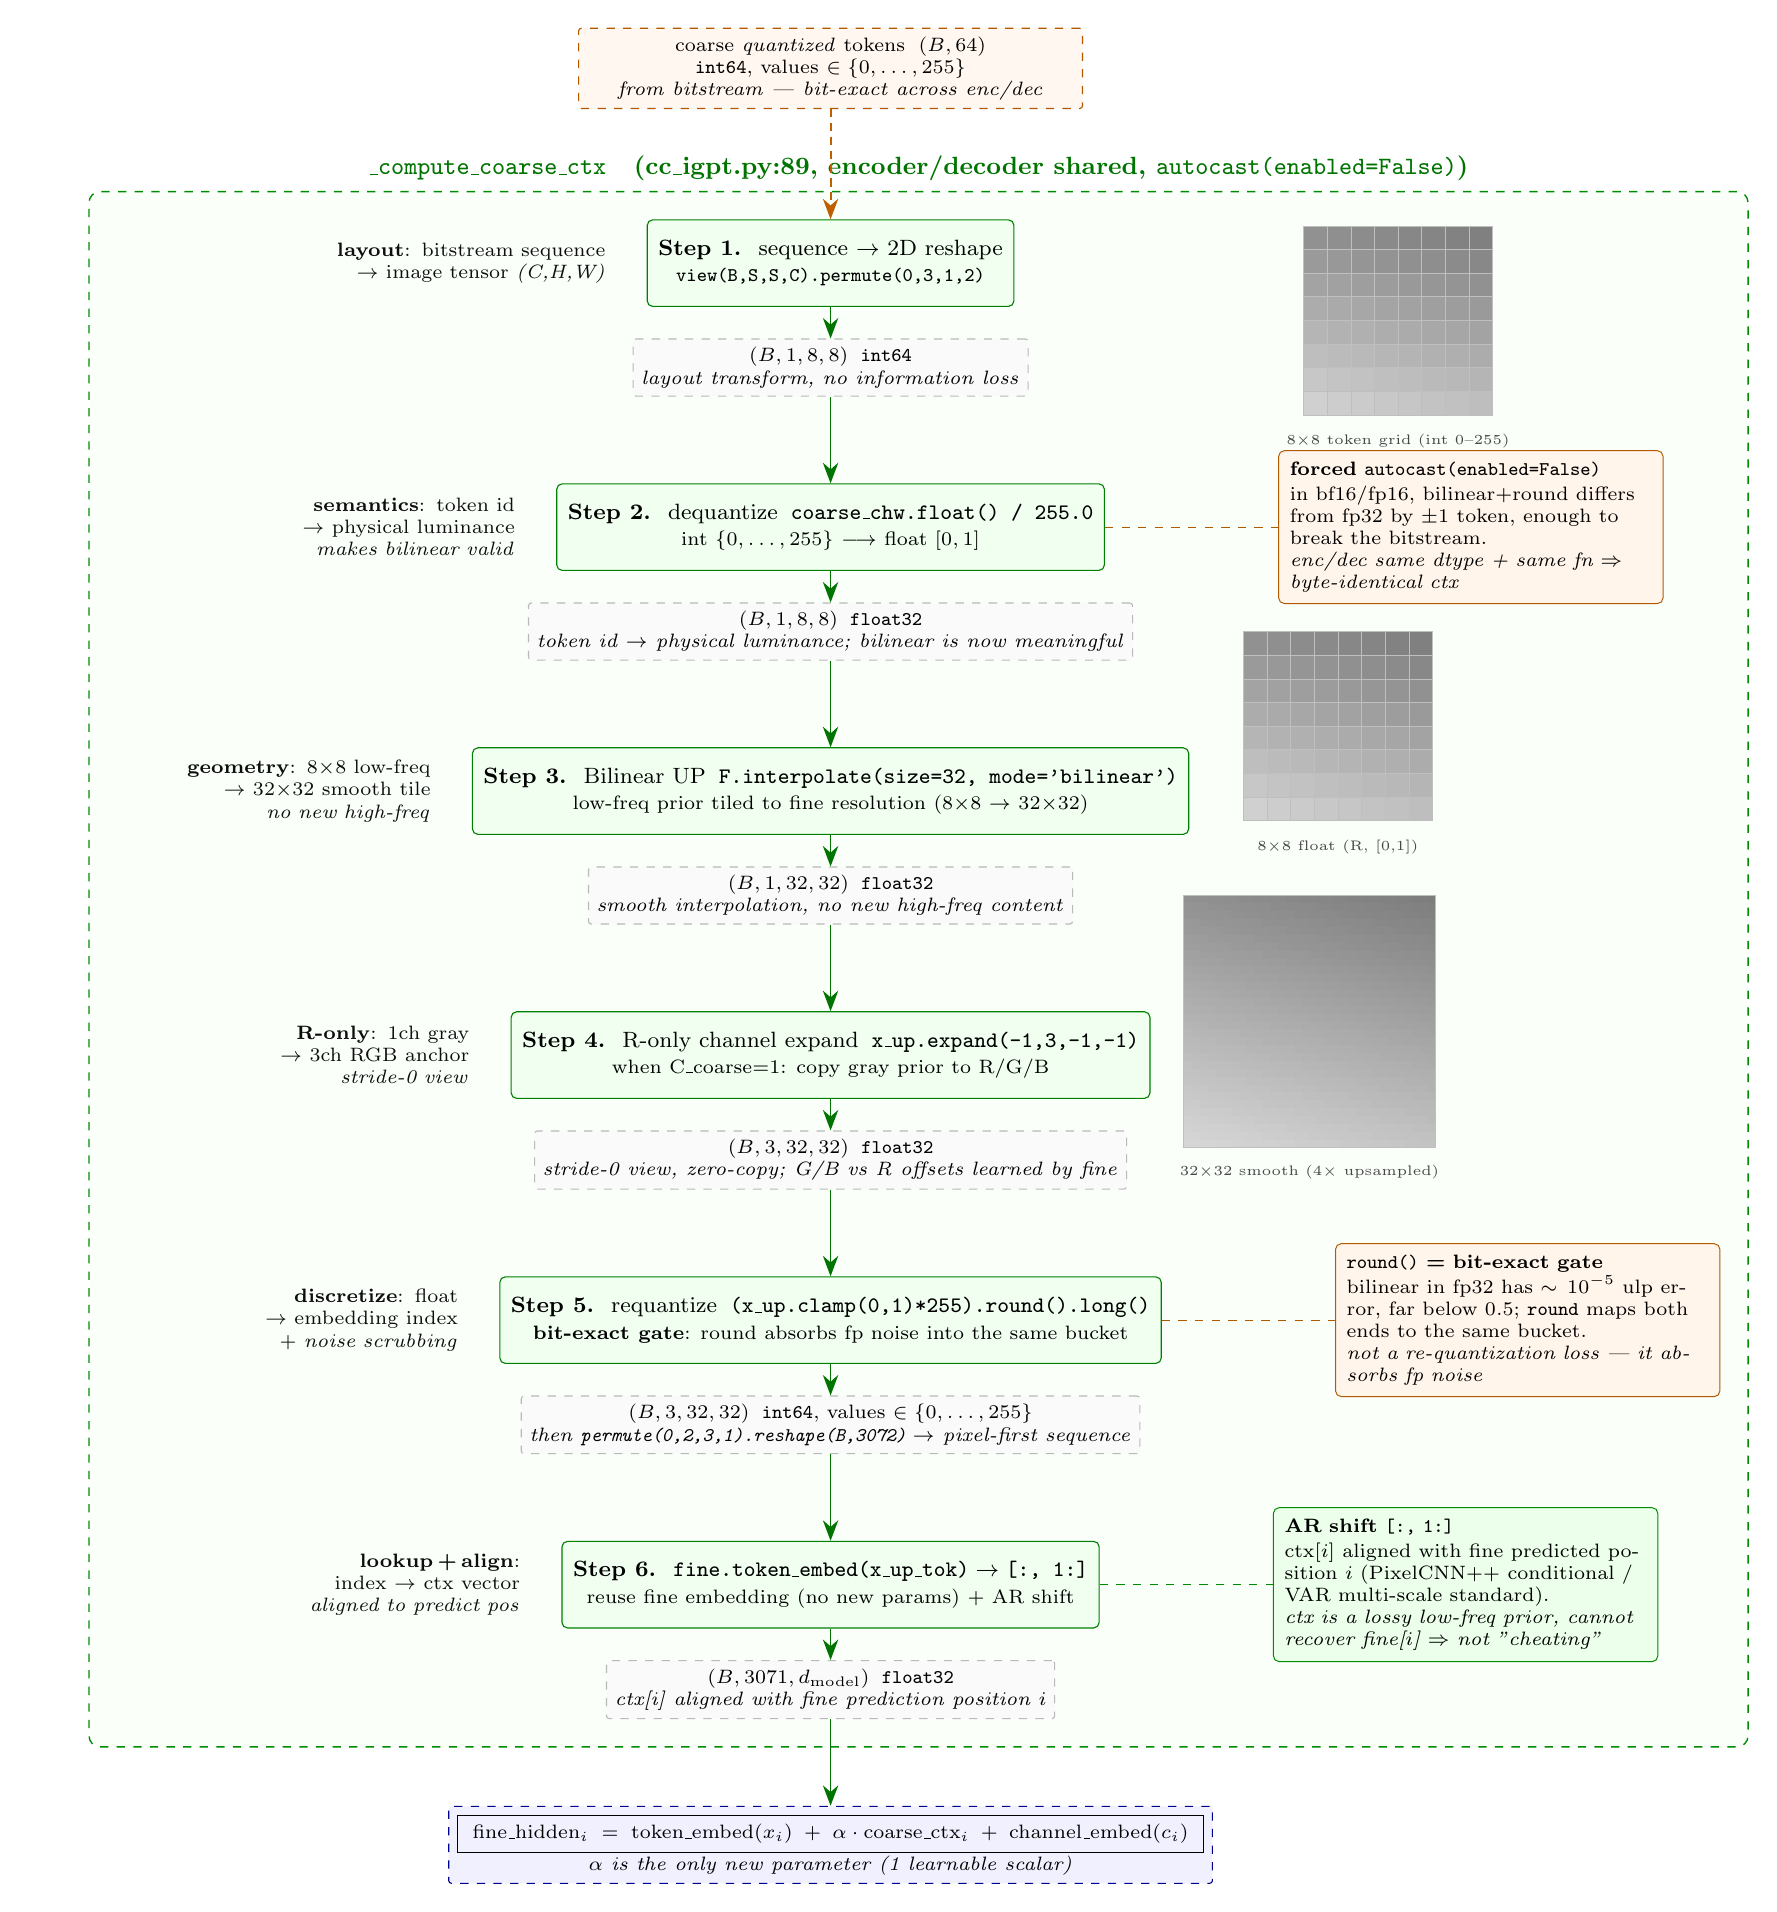
\begin{tikzpicture}[
    font=\footnotesize,
    >={Stealth[length=2.6mm]},
    node distance=10mm and 14mm,
    % ---- step blocks ----
    stepbox/.style ={draw, rounded corners=2pt, align=center,
                     minimum height=11mm, minimum width=46mm,
                     inner sep=4pt, fill=green!6, draw=green!50!black,
                     line width=0.4pt},
    % ---- tensor description (dashed gray) ----
    tensor/.style  ={draw, dashed, rounded corners=1pt, align=center,
                     fill=gray!4, draw=gray!55, font=\scriptsize,
                     inner sep=3pt, minimum width=46mm},
    % ---- mini grid cells ----
    gcell/.style   ={draw=gray!50, line width=0.18pt},
    gridlbl/.style ={font=\tiny, gray!55!black},
    % ---- callouts ----
    callout/.style ={draw=orange!70!black, rounded corners=2pt,
                     fill=orange!8, align=left, font=\scriptsize,
                     inner sep=4pt, line width=0.35pt},
    % ---- arrows ----
    flow/.style    ={->, line width=0.55pt, green!45!black},
    biteq/.style   ={->, line width=0.7pt, orange!75!black, densely dashed},
]

% =========================================================
% TOP: bitstream entry (input is integer tokens)
% =========================================================
\node[tensor, fill=orange!6, draw=orange!70!black, minimum width=64mm]
     (intok) {coarse \emph{quantized} tokens \;$(B,64)$\\
              \texttt{int64}, values $\in\{0,\dots,255\}$\\
              \textit{from bitstream --- bit-exact across enc/dec}};

% Step 0 mini-vis: 8x8 integer heatmap (true coarse spatial size; no in-cell labels)
\begin{scope}[shift={($(intok.east)+(28mm,-20mm)$)}, scale=0.30]
  \foreach \r in {0,...,7}{
    \foreach \c in {0,...,7}{
      \pgfmathtruncatemacro{\g}{round((220 - 18*\r + 5*\c)/2.55)}
      \fill[gray!\g!white] (\c,-\r) rectangle ++(1,-1);
      \draw[gcell] (\c,-\r) rectangle ++(1,-1);
    }
  }
  \node[gridlbl, anchor=north] at (4,-8.4) {$8{\times}8$ token grid (int 0--255)};
\end{scope}

% =========================================================
% Step 1 -- sequence to 2D reshape
% =========================================================
\node[stepbox, below=14mm of intok] (s1)
     {\textbf{Step 1.} \;sequence $\to$ 2D reshape\\
      \scriptsize\texttt{view(B,S,S,C).permute(0,3,1,2)}};
\node[tensor, below=4mm of s1] (t1)
     {$(B,1,8,8)$\;\;\texttt{int64}\\
      \textit{layout transform, no information loss}};

% =========================================================
% Step 2 -- dequantize /255 (int -> float [0,1])
% =========================================================
\node[stepbox, below=11mm of t1] (s2)
     {\textbf{Step 2.} \;dequantize\;\;\texttt{coarse\_chw.float() / 255.0}\\
      \scriptsize int $\{0,\dots,255\}$ $\longrightarrow$ float $[0,1]$};
\node[tensor, below=4mm of s2] (t2)
     {$(B,1,8,8)$\;\;\texttt{float32}\\
      \textit{token id $\to$ physical luminance; bilinear is now meaningful}};

% Step 2 mini-vis: 8x8 float heatmap (no in-cell labels to avoid clutter)
\begin{scope}[shift={($(t2.east)+(14mm,0)$)}, scale=0.30]
  \foreach \r in {0,...,7}{
    \foreach \c in {0,...,7}{
      \pgfmathtruncatemacro{\g}{round(86 - 7*\r + 2*\c)}
      \fill[gray!\g!white] (\c,-\r) rectangle ++(1,-1);
      \draw[gcell] (\c,-\r) rectangle ++(1,-1);
    }
  }
  \node[gridlbl, anchor=north] at (4,-8.4) {$8{\times}8$ float (R, [0,1])};
\end{scope}

% =========================================================
% Step 3 -- bilinear up 4x4 -> 32x32
% =========================================================
\node[stepbox, below=11mm of t2] (s3)
     {\textbf{Step 3.} \;Bilinear UP\;\;\texttt{F.interpolate(size=32, mode='bilinear')}\\
      \scriptsize low-freq prior tiled to fine resolution (8$\times$8 $\to$ 32$\times$32)};
\node[tensor, below=4mm of s3] (t3)
     {$(B,1,32,32)$\;\;\texttt{float32}\\
      \textit{smooth interpolation, no new high-freq content}};

% Step 3 mini-vis: 32x32 smooth schematic (larger than 8x8 to reflect 4x upsampling)
\begin{scope}[shift={($(t3.east)+(14mm,0)$)}, scale=0.10]
  \foreach \r in {0,...,31}{
    \foreach \c in {0,...,31}{
      \pgfmathtruncatemacro{\valc}%
        {round(86 - 7*(\r/4) + 2*(\c/4))}
      \fill[gray!\valc!white] (\c,-\r) rectangle ++(1,-1);
    }
  }
  \draw[gcell, line width=0.15pt] (0,-32) rectangle (32,0);
  \node[gridlbl, anchor=north] at (16,-33) {$32{\times}32$ smooth (4$\times$ upsampled)};
\end{scope}

% =========================================================
% Step 4 -- R-only expand 1ch -> 3ch
% =========================================================
\node[stepbox, below=11mm of t3] (s4)
     {\textbf{Step 4.} \;R-only channel expand\;\;\texttt{x\_up.expand(-1,3,-1,-1)}\\
      \scriptsize when C\_coarse$=$1: copy gray prior to R/G/B};
\node[tensor, below=4mm of s4] (t4)
     {$(B,3,32,32)$\;\;\texttt{float32}\\
      \textit{stride-0 view, zero-copy; G/B vs R offsets learned by fine}};

% =========================================================
% Step 5 -- requantize (x255 + round + long)
% =========================================================
\node[stepbox, below=11mm of t4] (s5)
     {\textbf{Step 5.} \;requantize\;\;\texttt{(x\_up.clamp(0,1)*255).round().long()}\\
      \scriptsize\textbf{bit-exact gate}: round absorbs fp noise into the same bucket};
\node[tensor, below=4mm of s5] (t5)
     {$(B,3,32,32)$\;\;\texttt{int64}, values $\in\{0,\dots,255\}$\\
      \textit{then \texttt{permute(0,2,3,1).reshape(B,3072)}\;$\to$ pixel-first sequence}};

% =========================================================
% Step 6 -- embedding lookup + AR shift
% =========================================================
\node[stepbox, below=11mm of t5] (s6)
     {\textbf{Step 6.} \;\texttt{fine.token\_embed(x\_up\_tok)}\;$\to$\;\texttt{[:, 1:]}\\
      \scriptsize reuse fine embedding (no new params) + AR shift};
\node[tensor, below=4mm of s6] (t6)
     {$(B,3071,d_{\text{model}})$\;\;\texttt{float32}\\
      \textit{ctx[i] aligned with fine prediction position $i$}};

% =========================================================
% OUTPUT: additive ctx injected into fine
% =========================================================
\node[tensor, fill=blue!6, draw=blue!55!black, below=11mm of t6,
      minimum width=72mm]
     (out) {$\boxed{\;\text{fine\_hidden}_i \;=\; \text{token\_embed}(x_i)
              \;+\;\alpha\cdot\text{coarse\_ctx}_i\;+\;\text{channel\_embed}(c_i)\;}$\\
            \scriptsize\textit{$\alpha$ is the only new parameter (1 learnable scalar)}};

% =========================================================
% Main flow arrows
% =========================================================
\draw[biteq] (intok) -- (s1);
\draw[flow]  (s1) -- (t1);
\draw[flow]  (t1) -- (s2);
\draw[flow]  (s2) -- (t2);
\draw[flow]  (t2) -- (s3);
\draw[flow]  (s3) -- (t3);
\draw[flow]  (t3) -- (s4);
\draw[flow]  (s4) -- (t4);
\draw[flow]  (t4) -- (s5);
\draw[flow]  (s5) -- (t5);
\draw[flow]  (t5) -- (s6);
\draw[flow]  (s6) -- (t6);
\draw[flow]  (t6) -- (out);

% =========================================================
% RIGHT-side callout bubbles (key invariants)
% =========================================================
% (A) autocast(enabled=False)
\node[callout, right=22mm of s2, anchor=west, text width=46mm]
     (caA) {\textbf{forced \texttt{autocast(enabled=False)}}\\[1pt]
            in bf16/fp16, bilinear+round differs from fp32 by $\pm 1$ token,
            enough to break the bitstream.\\
            \textit{enc/dec same dtype + same fn $\Rightarrow$ byte-identical ctx}};
\draw[orange!70!black, dashed, line width=0.35pt]
     (s2.east) -- (caA.west);

% (B) round() = bit-exact gate
\node[callout, right=22mm of s5, anchor=west, text width=46mm]
     (caB) {\textbf{\texttt{round()} = bit-exact gate}\\[1pt]
            bilinear in fp32 has $\sim 10^{-5}$ ulp error, far below $0.5$;
            \texttt{round} maps both ends to the same bucket.\\
            \textit{not a re-quantization loss --- it absorbs fp noise}};
\draw[orange!70!black, dashed, line width=0.35pt]
     (s5.east) -- (caB.west);

% (C) AR shift semantics
\node[callout, right=22mm of s6, anchor=west, text width=46mm,
      fill=green!8, draw=green!55!black]
     (caC) {\textbf{AR shift \texttt{[:, 1:]}}\\[1pt]
            ctx[$i$] aligned with fine predicted position $i$
            (PixelCNN++ conditional / VAR multi-scale standard).\\
            \textit{ctx is a lossy low-freq prior, cannot recover fine[$i$]
            $\Rightarrow$ not "cheating"}};
\draw[green!55!black, dashed, line width=0.35pt]
     (s6.east) -- (caC.west);

% =========================================================
% LEFT-side per-step semantics annotations
% =========================================================
\node[font=\scriptsize, gray!10!black, anchor=east, align=right,
      text width=50mm] (n1) at ($(s1.west)+(-4mm,0)$)
     {\textbf{layout}: bitstream sequence\\$\to$ image tensor \textit{(C,H,W)}};
\node[font=\scriptsize, gray!10!black, anchor=east, align=right,
      text width=50mm] (n2) at ($(s2.west)+(-4mm,0)$)
     {\textbf{semantics}: token id\\$\to$ physical luminance\\\textit{makes bilinear valid}};
\node[font=\scriptsize, gray!10!black, anchor=east, align=right,
      text width=50mm] (n3) at ($(s3.west)+(-4mm,0)$)
     {\textbf{geometry}: 8$\times$8 low-freq\\$\to$ 32$\times$32 smooth tile\\\textit{no new high-freq}};
\node[font=\scriptsize, gray!10!black, anchor=east, align=right,
      text width=50mm] (n4) at ($(s4.west)+(-4mm,0)$)
     {\textbf{R-only}: 1ch gray\\$\to$ 3ch RGB anchor\\\textit{stride-0 view}};
\node[font=\scriptsize, gray!10!black, anchor=east, align=right,
      text width=50mm] (n5) at ($(s5.west)+(-4mm,0)$)
     {\textbf{discretize}: float\\$\to$ embedding index\\\textit{$+$ noise scrubbing}};
\node[font=\scriptsize, gray!10!black, anchor=east, align=right,
      text width=50mm] (n6) at ($(s6.west)+(-4mm,0)$)
     {\textbf{lookup\,+\,align}:\\index $\to$ ctx vector\\\textit{aligned to predict pos}};

% =========================================================
% Background frame: whole _compute_coarse_ctx function
% =========================================================
\begin{pgfonlayer}{background}
  \node[draw=green!55!black, dashed, rounded corners=4pt,
        fill=green!2, line width=0.5pt, inner sep=10pt,
        fit=(s1)(s6)(t1)(t6)(caA)(caB)(caC)(n1)(n6),
        label={[green!45!black, font=\small\bfseries]above:%
              \texttt{\_compute\_coarse\_ctx} \;
              (cc\_igpt.py:89, encoder/decoder shared,
               \texttt{autocast(enabled=False)})}]
        (fnbox) {};
\end{pgfonlayer}

\end{tikzpicture}
\end{document}

%
% 与 ccigpt_arch.tex（系统图）配套：本图把 _compute_coarse_ctx 的 6 步管线
% 在「张量形状 + dtype + 可视化网格」三个层面全部具象化。
\documentclass[tikz,border=10pt]{standalone}
\usepackage{tikz}
\usepackage{amsmath,amssymb}
\usepackage{xcolor}
\usetikzlibrary{positioning,arrows.meta,calc,fit,backgrounds,shapes.geometric,
                decorations.pathreplacing,patterns}

\begin{document}
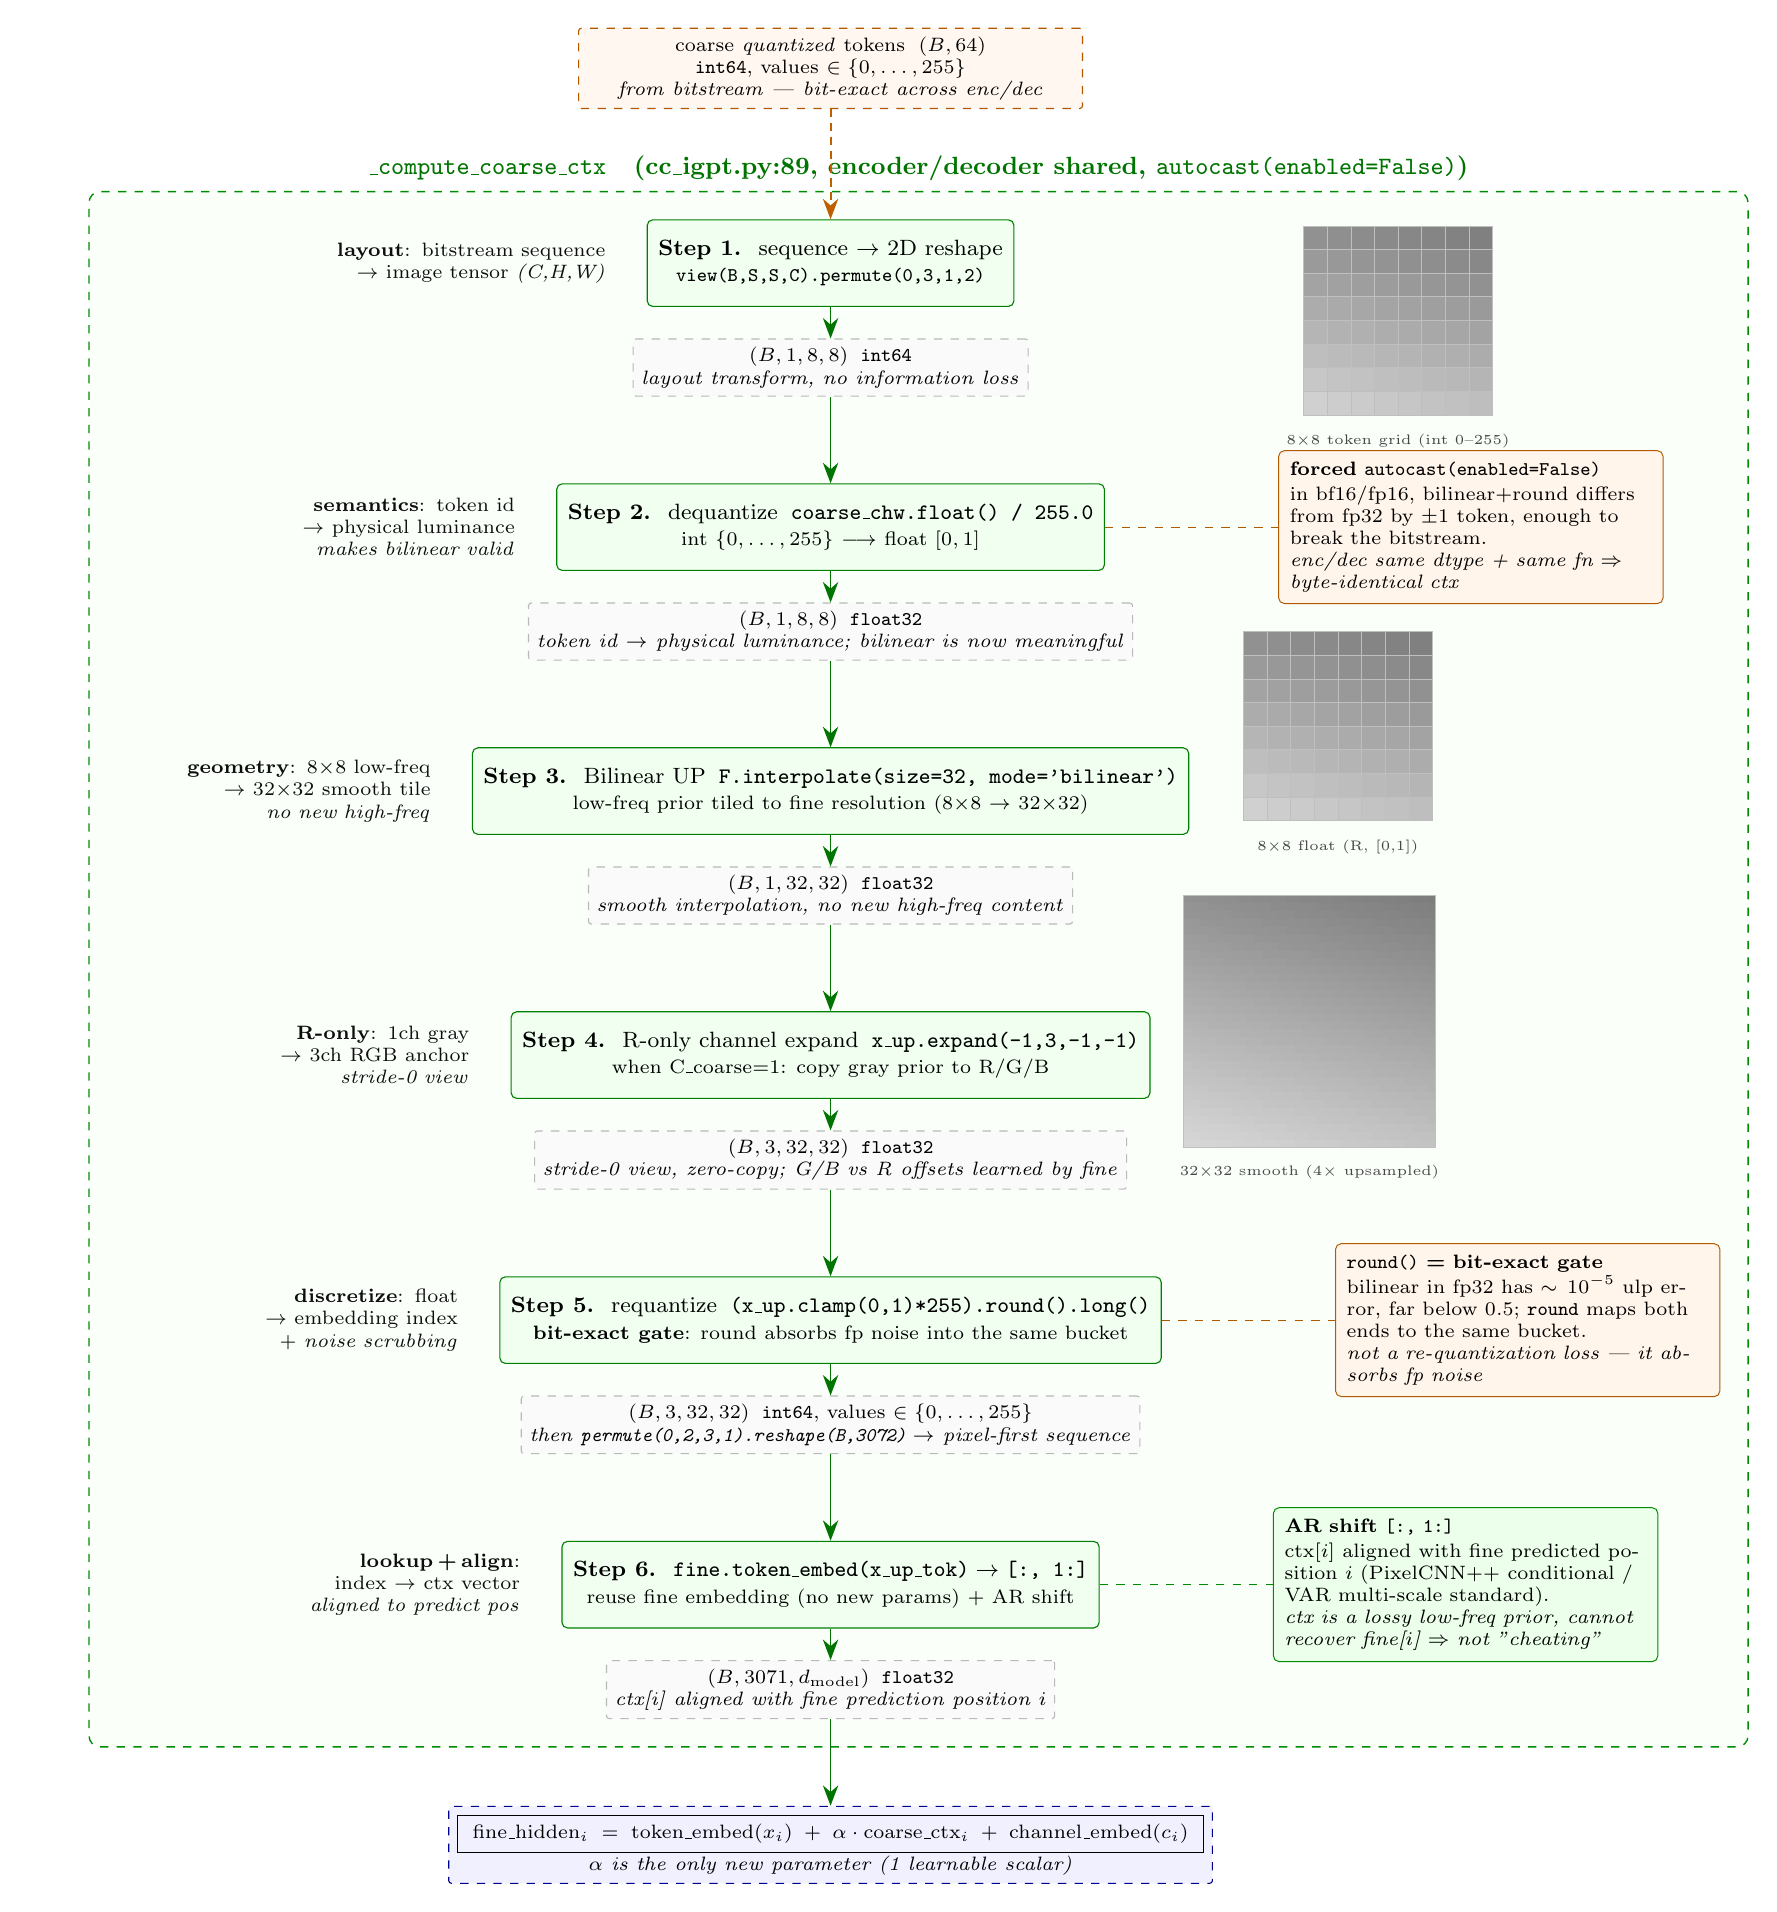
\begin{tikzpicture}[
    font=\footnotesize,
    >={Stealth[length=2.6mm]},
    node distance=10mm and 14mm,
    % ---- step blocks ----
    stepbox/.style ={draw, rounded corners=2pt, align=center,
                     minimum height=11mm, minimum width=46mm,
                     inner sep=4pt, fill=green!6, draw=green!50!black,
                     line width=0.4pt},
    % ---- tensor description (dashed gray) ----
    tensor/.style  ={draw, dashed, rounded corners=1pt, align=center,
                     fill=gray!4, draw=gray!55, font=\scriptsize,
                     inner sep=3pt, minimum width=46mm},
    % ---- mini grid cells ----
    gcell/.style   ={draw=gray!50, line width=0.18pt},
    gridlbl/.style ={font=\tiny, gray!55!black},
    % ---- callouts ----
    callout/.style ={draw=orange!70!black, rounded corners=2pt,
                     fill=orange!8, align=left, font=\scriptsize,
                     inner sep=4pt, line width=0.35pt},
    % ---- arrows ----
    flow/.style    ={->, line width=0.55pt, green!45!black},
    biteq/.style   ={->, line width=0.7pt, orange!75!black, densely dashed},
]

% =========================================================
% TOP: bitstream entry (input is integer tokens)
% =========================================================
\node[tensor, fill=orange!6, draw=orange!70!black, minimum width=64mm]
     (intok) {coarse \emph{quantized} tokens \;$(B,64)$\\
              \texttt{int64}, values $\in\{0,\dots,255\}$\\
              \textit{from bitstream --- bit-exact across enc/dec}};

% Step 0 mini-vis: 8x8 integer heatmap (true coarse spatial size; no in-cell labels)
\begin{scope}[shift={($(intok.east)+(28mm,-20mm)$)}, scale=0.30]
  \foreach \r in {0,...,7}{
    \foreach \c in {0,...,7}{
      \pgfmathtruncatemacro{\g}{round((220 - 18*\r + 5*\c)/2.55)}
      \fill[gray!\g!white] (\c,-\r) rectangle ++(1,-1);
      \draw[gcell] (\c,-\r) rectangle ++(1,-1);
    }
  }
  \node[gridlbl, anchor=north] at (4,-8.4) {$8{\times}8$ token grid (int 0--255)};
\end{scope}

% =========================================================
% Step 1 -- sequence to 2D reshape
% =========================================================
\node[stepbox, below=14mm of intok] (s1)
     {\textbf{Step 1.} \;sequence $\to$ 2D reshape\\
      \scriptsize\texttt{view(B,S,S,C).permute(0,3,1,2)}};
\node[tensor, below=4mm of s1] (t1)
     {$(B,1,8,8)$\;\;\texttt{int64}\\
      \textit{layout transform, no information loss}};

% =========================================================
% Step 2 -- dequantize /255 (int -> float [0,1])
% =========================================================
\node[stepbox, below=11mm of t1] (s2)
     {\textbf{Step 2.} \;dequantize\;\;\texttt{coarse\_chw.float() / 255.0}\\
      \scriptsize int $\{0,\dots,255\}$ $\longrightarrow$ float $[0,1]$};
\node[tensor, below=4mm of s2] (t2)
     {$(B,1,8,8)$\;\;\texttt{float32}\\
      \textit{token id $\to$ physical luminance; bilinear is now meaningful}};

% Step 2 mini-vis: 8x8 float heatmap (no in-cell labels to avoid clutter)
\begin{scope}[shift={($(t2.east)+(14mm,0)$)}, scale=0.30]
  \foreach \r in {0,...,7}{
    \foreach \c in {0,...,7}{
      \pgfmathtruncatemacro{\g}{round(86 - 7*\r + 2*\c)}
      \fill[gray!\g!white] (\c,-\r) rectangle ++(1,-1);
      \draw[gcell] (\c,-\r) rectangle ++(1,-1);
    }
  }
  \node[gridlbl, anchor=north] at (4,-8.4) {$8{\times}8$ float (R, [0,1])};
\end{scope}

% =========================================================
% Step 3 -- bilinear up 4x4 -> 32x32
% =========================================================
\node[stepbox, below=11mm of t2] (s3)
     {\textbf{Step 3.} \;Bilinear UP\;\;\texttt{F.interpolate(size=32, mode='bilinear')}\\
      \scriptsize low-freq prior tiled to fine resolution (8$\times$8 $\to$ 32$\times$32)};
\node[tensor, below=4mm of s3] (t3)
     {$(B,1,32,32)$\;\;\texttt{float32}\\
      \textit{smooth interpolation, no new high-freq content}};

% Step 3 mini-vis: 32x32 smooth schematic (larger than 8x8 to reflect 4x upsampling)
\begin{scope}[shift={($(t3.east)+(14mm,0)$)}, scale=0.10]
  \foreach \r in {0,...,31}{
    \foreach \c in {0,...,31}{
      \pgfmathtruncatemacro{\valc}%
        {round(86 - 7*(\r/4) + 2*(\c/4))}
      \fill[gray!\valc!white] (\c,-\r) rectangle ++(1,-1);
    }
  }
  \draw[gcell, line width=0.15pt] (0,-32) rectangle (32,0);
  \node[gridlbl, anchor=north] at (16,-33) {$32{\times}32$ smooth (4$\times$ upsampled)};
\end{scope}

% =========================================================
% Step 4 -- R-only expand 1ch -> 3ch
% =========================================================
\node[stepbox, below=11mm of t3] (s4)
     {\textbf{Step 4.} \;R-only channel expand\;\;\texttt{x\_up.expand(-1,3,-1,-1)}\\
      \scriptsize when C\_coarse$=$1: copy gray prior to R/G/B};
\node[tensor, below=4mm of s4] (t4)
     {$(B,3,32,32)$\;\;\texttt{float32}\\
      \textit{stride-0 view, zero-copy; G/B vs R offsets learned by fine}};

% =========================================================
% Step 5 -- requantize (x255 + round + long)
% =========================================================
\node[stepbox, below=11mm of t4] (s5)
     {\textbf{Step 5.} \;requantize\;\;\texttt{(x\_up.clamp(0,1)*255).round().long()}\\
      \scriptsize\textbf{bit-exact gate}: round absorbs fp noise into the same bucket};
\node[tensor, below=4mm of s5] (t5)
     {$(B,3,32,32)$\;\;\texttt{int64}, values $\in\{0,\dots,255\}$\\
      \textit{then \texttt{permute(0,2,3,1).reshape(B,3072)}\;$\to$ pixel-first sequence}};

% =========================================================
% Step 6 -- embedding lookup + AR shift
% =========================================================
\node[stepbox, below=11mm of t5] (s6)
     {\textbf{Step 6.} \;\texttt{fine.token\_embed(x\_up\_tok)}\;$\to$\;\texttt{[:, 1:]}\\
      \scriptsize reuse fine embedding (no new params) + AR shift};
\node[tensor, below=4mm of s6] (t6)
     {$(B,3071,d_{\text{model}})$\;\;\texttt{float32}\\
      \textit{ctx[i] aligned with fine prediction position $i$}};

% =========================================================
% OUTPUT: additive ctx injected into fine
% =========================================================
\node[tensor, fill=blue!6, draw=blue!55!black, below=11mm of t6,
      minimum width=72mm]
     (out) {$\boxed{\;\text{fine\_hidden}_i \;=\; \text{token\_embed}(x_i)
              \;+\;\alpha\cdot\text{coarse\_ctx}_i\;+\;\text{channel\_embed}(c_i)\;}$\\
            \scriptsize\textit{$\alpha$ is the only new parameter (1 learnable scalar)}};

% =========================================================
% Main flow arrows
% =========================================================
\draw[biteq] (intok) -- (s1);
\draw[flow]  (s1) -- (t1);
\draw[flow]  (t1) -- (s2);
\draw[flow]  (s2) -- (t2);
\draw[flow]  (t2) -- (s3);
\draw[flow]  (s3) -- (t3);
\draw[flow]  (t3) -- (s4);
\draw[flow]  (s4) -- (t4);
\draw[flow]  (t4) -- (s5);
\draw[flow]  (s5) -- (t5);
\draw[flow]  (t5) -- (s6);
\draw[flow]  (s6) -- (t6);
\draw[flow]  (t6) -- (out);

% =========================================================
% RIGHT-side callout bubbles (key invariants)
% =========================================================
% (A) autocast(enabled=False)
\node[callout, right=22mm of s2, anchor=west, text width=46mm]
     (caA) {\textbf{forced \texttt{autocast(enabled=False)}}\\[1pt]
            in bf16/fp16, bilinear+round differs from fp32 by $\pm 1$ token,
            enough to break the bitstream.\\
            \textit{enc/dec same dtype + same fn $\Rightarrow$ byte-identical ctx}};
\draw[orange!70!black, dashed, line width=0.35pt]
     (s2.east) -- (caA.west);

% (B) round() = bit-exact gate
\node[callout, right=22mm of s5, anchor=west, text width=46mm]
     (caB) {\textbf{\texttt{round()} = bit-exact gate}\\[1pt]
            bilinear in fp32 has $\sim 10^{-5}$ ulp error, far below $0.5$;
            \texttt{round} maps both ends to the same bucket.\\
            \textit{not a re-quantization loss --- it absorbs fp noise}};
\draw[orange!70!black, dashed, line width=0.35pt]
     (s5.east) -- (caB.west);

% (C) AR shift semantics
\node[callout, right=22mm of s6, anchor=west, text width=46mm,
      fill=green!8, draw=green!55!black]
     (caC) {\textbf{AR shift \texttt{[:, 1:]}}\\[1pt]
            ctx[$i$] aligned with fine predicted position $i$
            (PixelCNN++ conditional / VAR multi-scale standard).\\
            \textit{ctx is a lossy low-freq prior, cannot recover fine[$i$]
            $\Rightarrow$ not "cheating"}};
\draw[green!55!black, dashed, line width=0.35pt]
     (s6.east) -- (caC.west);

% =========================================================
% LEFT-side per-step semantics annotations
% =========================================================
\node[font=\scriptsize, gray!10!black, anchor=east, align=right,
      text width=50mm] (n1) at ($(s1.west)+(-4mm,0)$)
     {\textbf{layout}: bitstream sequence\\$\to$ image tensor \textit{(C,H,W)}};
\node[font=\scriptsize, gray!10!black, anchor=east, align=right,
      text width=50mm] (n2) at ($(s2.west)+(-4mm,0)$)
     {\textbf{semantics}: token id\\$\to$ physical luminance\\\textit{makes bilinear valid}};
\node[font=\scriptsize, gray!10!black, anchor=east, align=right,
      text width=50mm] (n3) at ($(s3.west)+(-4mm,0)$)
     {\textbf{geometry}: 8$\times$8 low-freq\\$\to$ 32$\times$32 smooth tile\\\textit{no new high-freq}};
\node[font=\scriptsize, gray!10!black, anchor=east, align=right,
      text width=50mm] (n4) at ($(s4.west)+(-4mm,0)$)
     {\textbf{R-only}: 1ch gray\\$\to$ 3ch RGB anchor\\\textit{stride-0 view}};
\node[font=\scriptsize, gray!10!black, anchor=east, align=right,
      text width=50mm] (n5) at ($(s5.west)+(-4mm,0)$)
     {\textbf{discretize}: float\\$\to$ embedding index\\\textit{$+$ noise scrubbing}};
\node[font=\scriptsize, gray!10!black, anchor=east, align=right,
      text width=50mm] (n6) at ($(s6.west)+(-4mm,0)$)
     {\textbf{lookup\,+\,align}:\\index $\to$ ctx vector\\\textit{aligned to predict pos}};

% =========================================================
% Background frame: whole _compute_coarse_ctx function
% =========================================================
\begin{pgfonlayer}{background}
  \node[draw=green!55!black, dashed, rounded corners=4pt,
        fill=green!2, line width=0.5pt, inner sep=10pt,
        fit=(s1)(s6)(t1)(t6)(caA)(caB)(caC)(n1)(n6),
        label={[green!45!black, font=\small\bfseries]above:%
              \texttt{\_compute\_coarse\_ctx} \;
              (cc\_igpt.py:89, encoder/decoder shared,
               \texttt{autocast(enabled=False)})}]
        (fnbox) {};
\end{pgfonlayer}

\end{tikzpicture}
\end{document}

%
% 与 ccigpt_arch.tex（系统图）配套：本图把 _compute_coarse_ctx 的 6 步管线
% 在「张量形状 + dtype + 可视化网格」三个层面全部具象化。
\documentclass[tikz,border=10pt]{standalone}
\usepackage{tikz}
\usepackage{amsmath,amssymb}
\usepackage{xcolor}
\usetikzlibrary{positioning,arrows.meta,calc,fit,backgrounds,shapes.geometric,
                decorations.pathreplacing,patterns}

\begin{document}
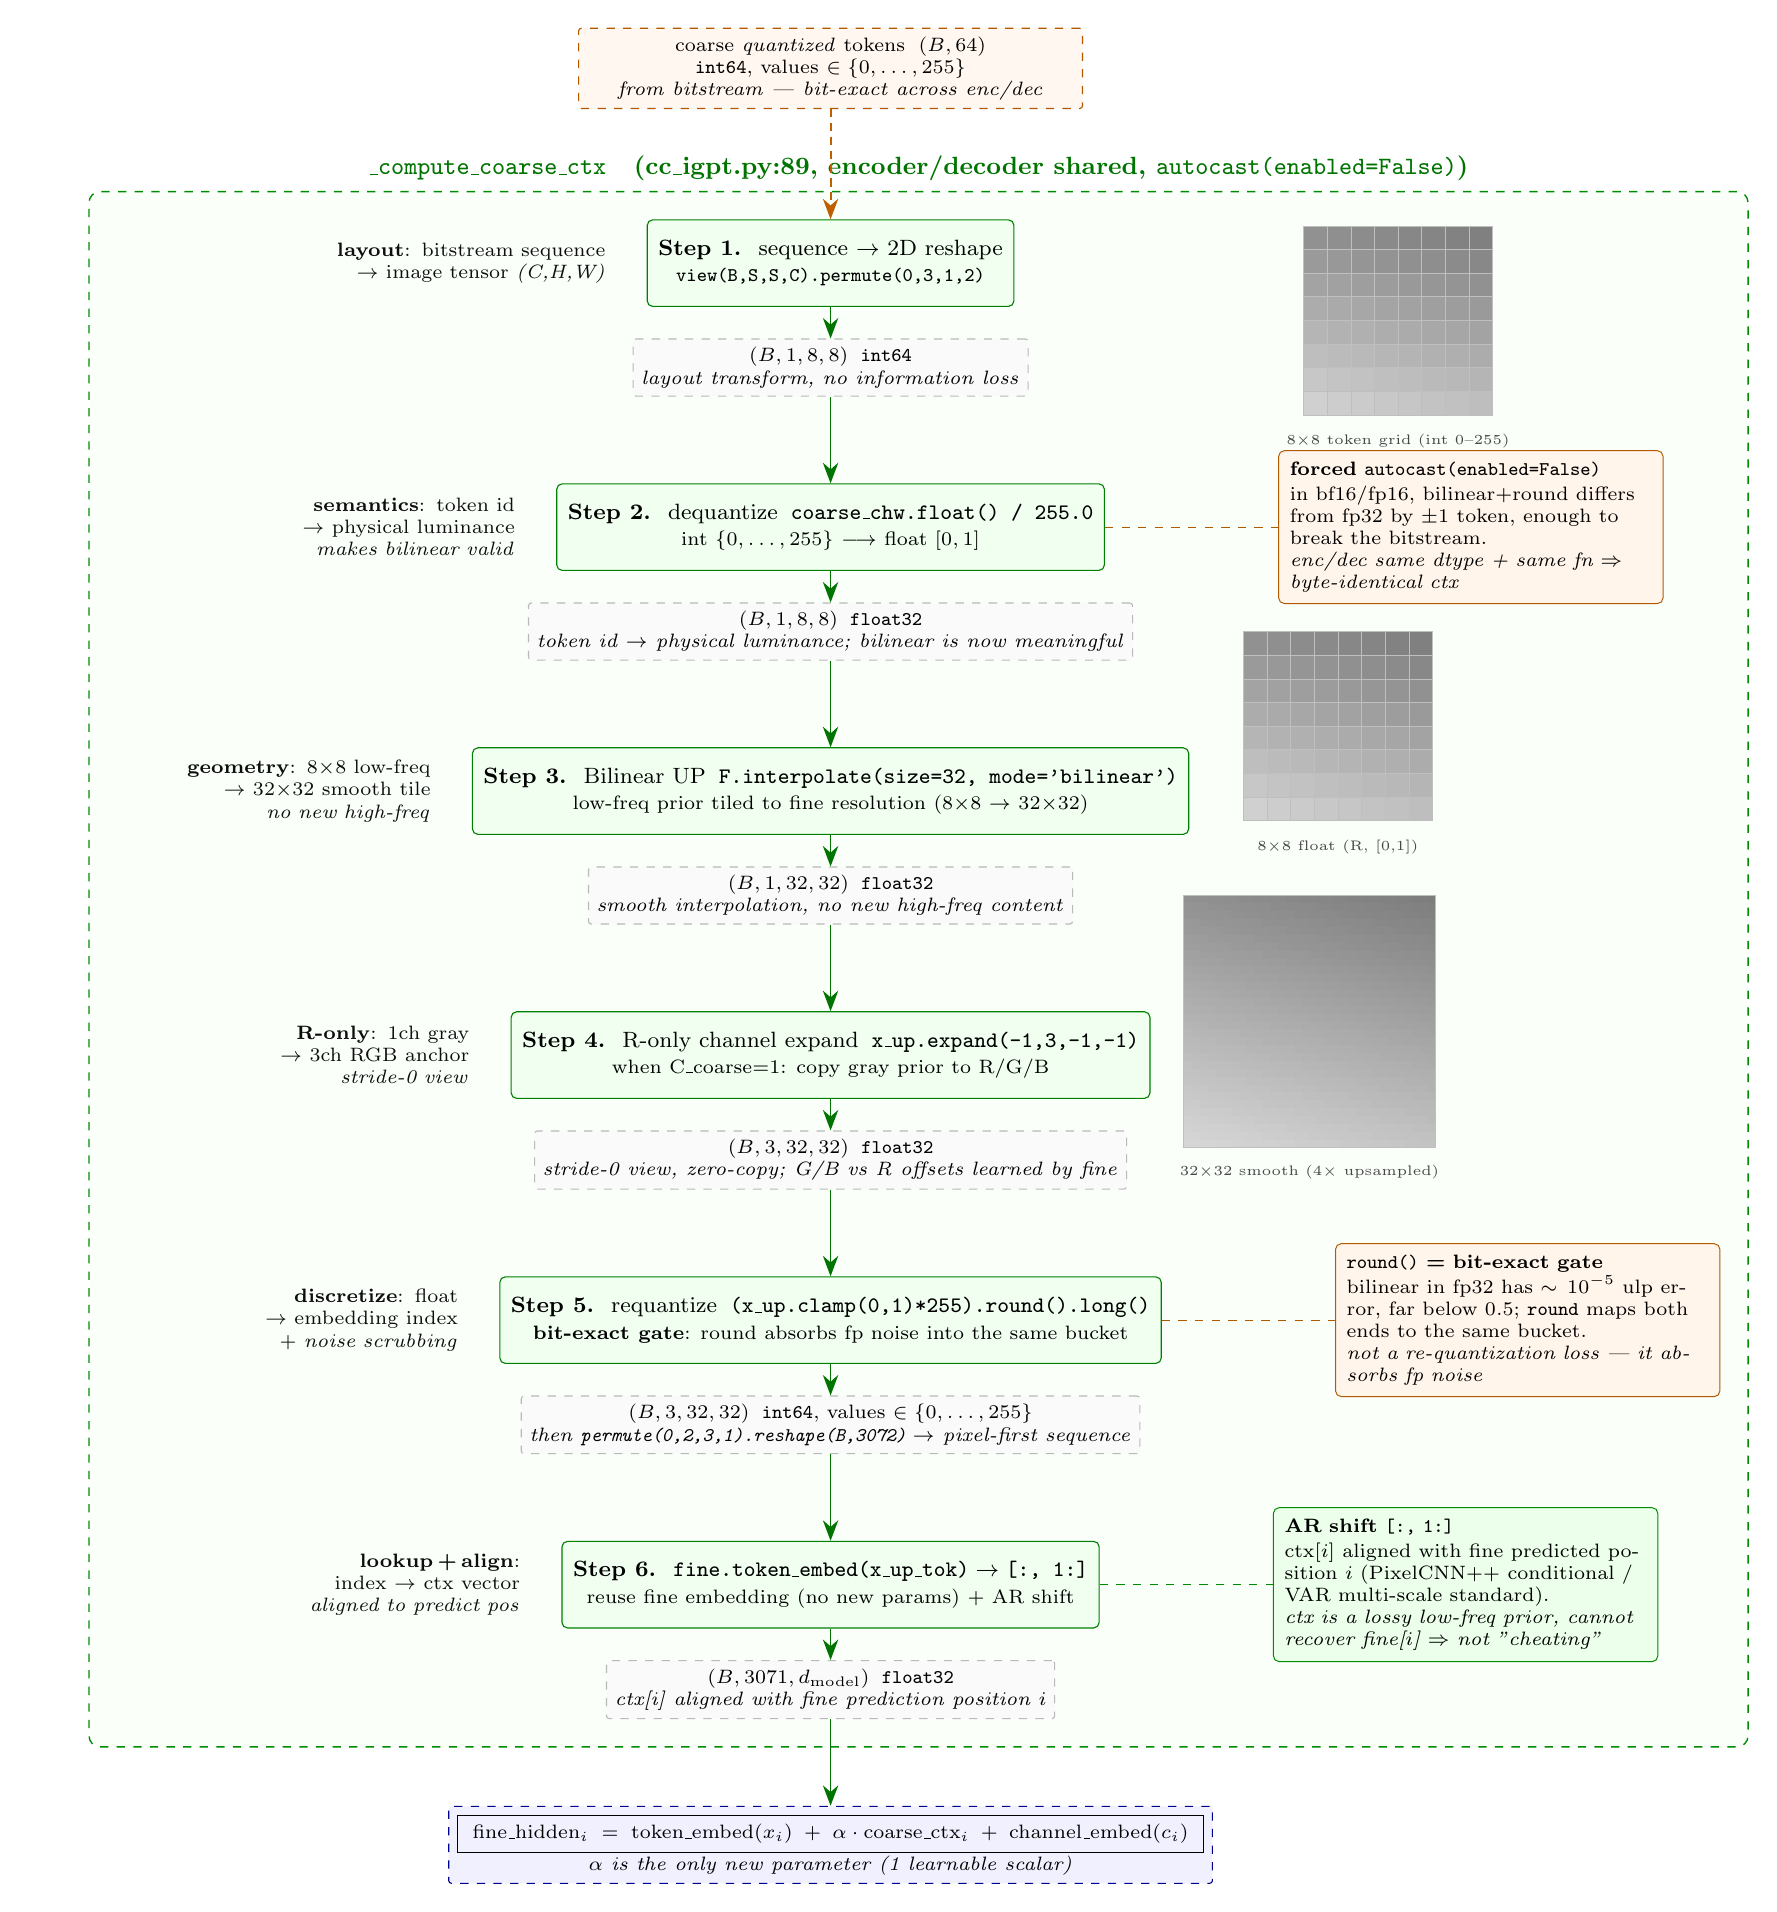
\begin{tikzpicture}[
    font=\footnotesize,
    >={Stealth[length=2.6mm]},
    node distance=10mm and 14mm,
    % ---- step blocks ----
    stepbox/.style ={draw, rounded corners=2pt, align=center,
                     minimum height=11mm, minimum width=46mm,
                     inner sep=4pt, fill=green!6, draw=green!50!black,
                     line width=0.4pt},
    % ---- tensor description (dashed gray) ----
    tensor/.style  ={draw, dashed, rounded corners=1pt, align=center,
                     fill=gray!4, draw=gray!55, font=\scriptsize,
                     inner sep=3pt, minimum width=46mm},
    % ---- mini grid cells ----
    gcell/.style   ={draw=gray!50, line width=0.18pt},
    gridlbl/.style ={font=\tiny, gray!55!black},
    % ---- callouts ----
    callout/.style ={draw=orange!70!black, rounded corners=2pt,
                     fill=orange!8, align=left, font=\scriptsize,
                     inner sep=4pt, line width=0.35pt},
    % ---- arrows ----
    flow/.style    ={->, line width=0.55pt, green!45!black},
    biteq/.style   ={->, line width=0.7pt, orange!75!black, densely dashed},
]

% =========================================================
% TOP: bitstream entry (input is integer tokens)
% =========================================================
\node[tensor, fill=orange!6, draw=orange!70!black, minimum width=64mm]
     (intok) {coarse \emph{quantized} tokens \;$(B,64)$\\
              \texttt{int64}, values $\in\{0,\dots,255\}$\\
              \textit{from bitstream --- bit-exact across enc/dec}};

% Step 0 mini-vis: 8x8 integer heatmap (true coarse spatial size; no in-cell labels)
\begin{scope}[shift={($(intok.east)+(28mm,-20mm)$)}, scale=0.30]
  \foreach \r in {0,...,7}{
    \foreach \c in {0,...,7}{
      \pgfmathtruncatemacro{\g}{round((220 - 18*\r + 5*\c)/2.55)}
      \fill[gray!\g!white] (\c,-\r) rectangle ++(1,-1);
      \draw[gcell] (\c,-\r) rectangle ++(1,-1);
    }
  }
  \node[gridlbl, anchor=north] at (4,-8.4) {$8{\times}8$ token grid (int 0--255)};
\end{scope}

% =========================================================
% Step 1 -- sequence to 2D reshape
% =========================================================
\node[stepbox, below=14mm of intok] (s1)
     {\textbf{Step 1.} \;sequence $\to$ 2D reshape\\
      \scriptsize\texttt{view(B,S,S,C).permute(0,3,1,2)}};
\node[tensor, below=4mm of s1] (t1)
     {$(B,1,8,8)$\;\;\texttt{int64}\\
      \textit{layout transform, no information loss}};

% =========================================================
% Step 2 -- dequantize /255 (int -> float [0,1])
% =========================================================
\node[stepbox, below=11mm of t1] (s2)
     {\textbf{Step 2.} \;dequantize\;\;\texttt{coarse\_chw.float() / 255.0}\\
      \scriptsize int $\{0,\dots,255\}$ $\longrightarrow$ float $[0,1]$};
\node[tensor, below=4mm of s2] (t2)
     {$(B,1,8,8)$\;\;\texttt{float32}\\
      \textit{token id $\to$ physical luminance; bilinear is now meaningful}};

% Step 2 mini-vis: 8x8 float heatmap (no in-cell labels to avoid clutter)
\begin{scope}[shift={($(t2.east)+(14mm,0)$)}, scale=0.30]
  \foreach \r in {0,...,7}{
    \foreach \c in {0,...,7}{
      \pgfmathtruncatemacro{\g}{round(86 - 7*\r + 2*\c)}
      \fill[gray!\g!white] (\c,-\r) rectangle ++(1,-1);
      \draw[gcell] (\c,-\r) rectangle ++(1,-1);
    }
  }
  \node[gridlbl, anchor=north] at (4,-8.4) {$8{\times}8$ float (R, [0,1])};
\end{scope}

% =========================================================
% Step 3 -- bilinear up 4x4 -> 32x32
% =========================================================
\node[stepbox, below=11mm of t2] (s3)
     {\textbf{Step 3.} \;Bilinear UP\;\;\texttt{F.interpolate(size=32, mode='bilinear')}\\
      \scriptsize low-freq prior tiled to fine resolution (8$\times$8 $\to$ 32$\times$32)};
\node[tensor, below=4mm of s3] (t3)
     {$(B,1,32,32)$\;\;\texttt{float32}\\
      \textit{smooth interpolation, no new high-freq content}};

% Step 3 mini-vis: 32x32 smooth schematic (larger than 8x8 to reflect 4x upsampling)
\begin{scope}[shift={($(t3.east)+(14mm,0)$)}, scale=0.10]
  \foreach \r in {0,...,31}{
    \foreach \c in {0,...,31}{
      \pgfmathtruncatemacro{\valc}%
        {round(86 - 7*(\r/4) + 2*(\c/4))}
      \fill[gray!\valc!white] (\c,-\r) rectangle ++(1,-1);
    }
  }
  \draw[gcell, line width=0.15pt] (0,-32) rectangle (32,0);
  \node[gridlbl, anchor=north] at (16,-33) {$32{\times}32$ smooth (4$\times$ upsampled)};
\end{scope}

% =========================================================
% Step 4 -- R-only expand 1ch -> 3ch
% =========================================================
\node[stepbox, below=11mm of t3] (s4)
     {\textbf{Step 4.} \;R-only channel expand\;\;\texttt{x\_up.expand(-1,3,-1,-1)}\\
      \scriptsize when C\_coarse$=$1: copy gray prior to R/G/B};
\node[tensor, below=4mm of s4] (t4)
     {$(B,3,32,32)$\;\;\texttt{float32}\\
      \textit{stride-0 view, zero-copy; G/B vs R offsets learned by fine}};

% =========================================================
% Step 5 -- requantize (x255 + round + long)
% =========================================================
\node[stepbox, below=11mm of t4] (s5)
     {\textbf{Step 5.} \;requantize\;\;\texttt{(x\_up.clamp(0,1)*255).round().long()}\\
      \scriptsize\textbf{bit-exact gate}: round absorbs fp noise into the same bucket};
\node[tensor, below=4mm of s5] (t5)
     {$(B,3,32,32)$\;\;\texttt{int64}, values $\in\{0,\dots,255\}$\\
      \textit{then \texttt{permute(0,2,3,1).reshape(B,3072)}\;$\to$ pixel-first sequence}};

% =========================================================
% Step 6 -- embedding lookup + AR shift
% =========================================================
\node[stepbox, below=11mm of t5] (s6)
     {\textbf{Step 6.} \;\texttt{fine.token\_embed(x\_up\_tok)}\;$\to$\;\texttt{[:, 1:]}\\
      \scriptsize reuse fine embedding (no new params) + AR shift};
\node[tensor, below=4mm of s6] (t6)
     {$(B,3071,d_{\text{model}})$\;\;\texttt{float32}\\
      \textit{ctx[i] aligned with fine prediction position $i$}};

% =========================================================
% OUTPUT: additive ctx injected into fine
% =========================================================
\node[tensor, fill=blue!6, draw=blue!55!black, below=11mm of t6,
      minimum width=72mm]
     (out) {$\boxed{\;\text{fine\_hidden}_i \;=\; \text{token\_embed}(x_i)
              \;+\;\alpha\cdot\text{coarse\_ctx}_i\;+\;\text{channel\_embed}(c_i)\;}$\\
            \scriptsize\textit{$\alpha$ is the only new parameter (1 learnable scalar)}};

% =========================================================
% Main flow arrows
% =========================================================
\draw[biteq] (intok) -- (s1);
\draw[flow]  (s1) -- (t1);
\draw[flow]  (t1) -- (s2);
\draw[flow]  (s2) -- (t2);
\draw[flow]  (t2) -- (s3);
\draw[flow]  (s3) -- (t3);
\draw[flow]  (t3) -- (s4);
\draw[flow]  (s4) -- (t4);
\draw[flow]  (t4) -- (s5);
\draw[flow]  (s5) -- (t5);
\draw[flow]  (t5) -- (s6);
\draw[flow]  (s6) -- (t6);
\draw[flow]  (t6) -- (out);

% =========================================================
% RIGHT-side callout bubbles (key invariants)
% =========================================================
% (A) autocast(enabled=False)
\node[callout, right=22mm of s2, anchor=west, text width=46mm]
     (caA) {\textbf{forced \texttt{autocast(enabled=False)}}\\[1pt]
            in bf16/fp16, bilinear+round differs from fp32 by $\pm 1$ token,
            enough to break the bitstream.\\
            \textit{enc/dec same dtype + same fn $\Rightarrow$ byte-identical ctx}};
\draw[orange!70!black, dashed, line width=0.35pt]
     (s2.east) -- (caA.west);

% (B) round() = bit-exact gate
\node[callout, right=22mm of s5, anchor=west, text width=46mm]
     (caB) {\textbf{\texttt{round()} = bit-exact gate}\\[1pt]
            bilinear in fp32 has $\sim 10^{-5}$ ulp error, far below $0.5$;
            \texttt{round} maps both ends to the same bucket.\\
            \textit{not a re-quantization loss --- it absorbs fp noise}};
\draw[orange!70!black, dashed, line width=0.35pt]
     (s5.east) -- (caB.west);

% (C) AR shift semantics
\node[callout, right=22mm of s6, anchor=west, text width=46mm,
      fill=green!8, draw=green!55!black]
     (caC) {\textbf{AR shift \texttt{[:, 1:]}}\\[1pt]
            ctx[$i$] aligned with fine predicted position $i$
            (PixelCNN++ conditional / VAR multi-scale standard).\\
            \textit{ctx is a lossy low-freq prior, cannot recover fine[$i$]
            $\Rightarrow$ not "cheating"}};
\draw[green!55!black, dashed, line width=0.35pt]
     (s6.east) -- (caC.west);

% =========================================================
% LEFT-side per-step semantics annotations
% =========================================================
\node[font=\scriptsize, gray!10!black, anchor=east, align=right,
      text width=50mm] (n1) at ($(s1.west)+(-4mm,0)$)
     {\textbf{layout}: bitstream sequence\\$\to$ image tensor \textit{(C,H,W)}};
\node[font=\scriptsize, gray!10!black, anchor=east, align=right,
      text width=50mm] (n2) at ($(s2.west)+(-4mm,0)$)
     {\textbf{semantics}: token id\\$\to$ physical luminance\\\textit{makes bilinear valid}};
\node[font=\scriptsize, gray!10!black, anchor=east, align=right,
      text width=50mm] (n3) at ($(s3.west)+(-4mm,0)$)
     {\textbf{geometry}: 8$\times$8 low-freq\\$\to$ 32$\times$32 smooth tile\\\textit{no new high-freq}};
\node[font=\scriptsize, gray!10!black, anchor=east, align=right,
      text width=50mm] (n4) at ($(s4.west)+(-4mm,0)$)
     {\textbf{R-only}: 1ch gray\\$\to$ 3ch RGB anchor\\\textit{stride-0 view}};
\node[font=\scriptsize, gray!10!black, anchor=east, align=right,
      text width=50mm] (n5) at ($(s5.west)+(-4mm,0)$)
     {\textbf{discretize}: float\\$\to$ embedding index\\\textit{$+$ noise scrubbing}};
\node[font=\scriptsize, gray!10!black, anchor=east, align=right,
      text width=50mm] (n6) at ($(s6.west)+(-4mm,0)$)
     {\textbf{lookup\,+\,align}:\\index $\to$ ctx vector\\\textit{aligned to predict pos}};

% =========================================================
% Background frame: whole _compute_coarse_ctx function
% =========================================================
\begin{pgfonlayer}{background}
  \node[draw=green!55!black, dashed, rounded corners=4pt,
        fill=green!2, line width=0.5pt, inner sep=10pt,
        fit=(s1)(s6)(t1)(t6)(caA)(caB)(caC)(n1)(n6),
        label={[green!45!black, font=\small\bfseries]above:%
              \texttt{\_compute\_coarse\_ctx} \;
              (cc\_igpt.py:89, encoder/decoder shared,
               \texttt{autocast(enabled=False)})}]
        (fnbox) {};
\end{pgfonlayer}

\end{tikzpicture}
\end{document}

%
% 与 ccigpt_arch.tex（系统图）配套：本图把 _compute_coarse_ctx 的 6 步管线
% 在「张量形状 + dtype + 可视化网格」三个层面全部具象化。
\documentclass[tikz,border=10pt]{standalone}
\usepackage{tikz}
\usepackage{amsmath,amssymb}
\usepackage{xcolor}
\usetikzlibrary{positioning,arrows.meta,calc,fit,backgrounds,shapes.geometric,
                decorations.pathreplacing,patterns}

\begin{document}
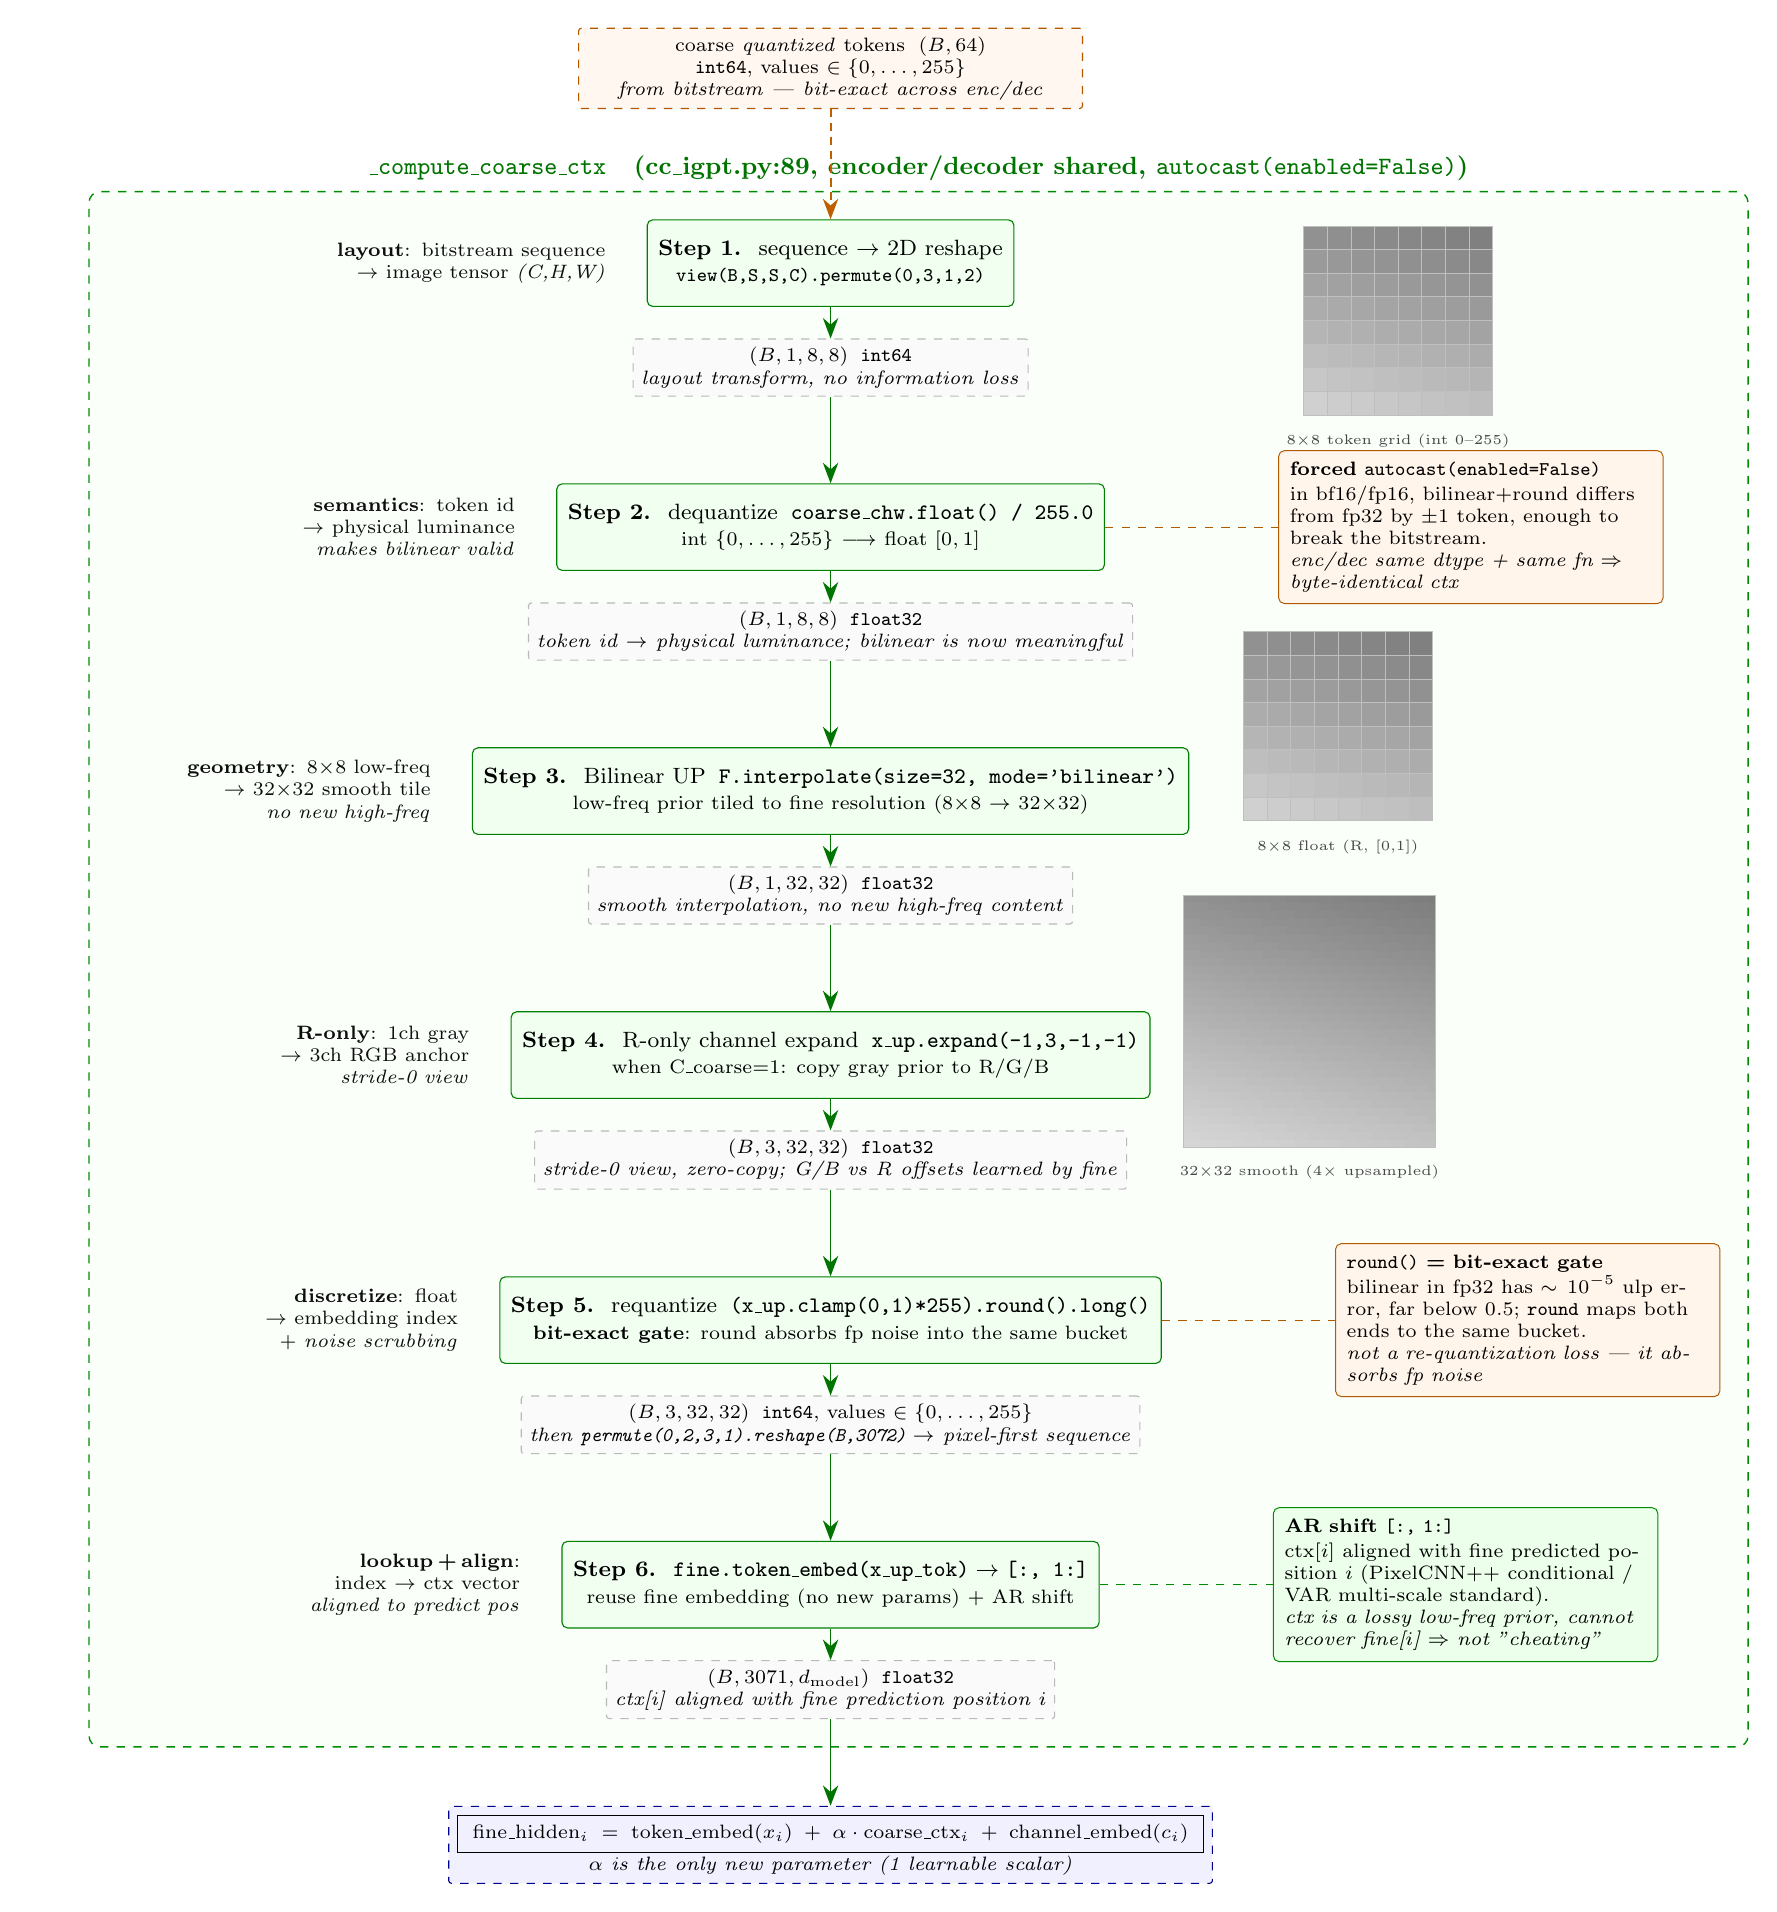
\begin{tikzpicture}[
    font=\footnotesize,
    >={Stealth[length=2.6mm]},
    node distance=10mm and 14mm,
    % ---- step blocks ----
    stepbox/.style ={draw, rounded corners=2pt, align=center,
                     minimum height=11mm, minimum width=46mm,
                     inner sep=4pt, fill=green!6, draw=green!50!black,
                     line width=0.4pt},
    % ---- tensor description (dashed gray) ----
    tensor/.style  ={draw, dashed, rounded corners=1pt, align=center,
                     fill=gray!4, draw=gray!55, font=\scriptsize,
                     inner sep=3pt, minimum width=46mm},
    % ---- mini grid cells ----
    gcell/.style   ={draw=gray!50, line width=0.18pt},
    gridlbl/.style ={font=\tiny, gray!55!black},
    % ---- callouts ----
    callout/.style ={draw=orange!70!black, rounded corners=2pt,
                     fill=orange!8, align=left, font=\scriptsize,
                     inner sep=4pt, line width=0.35pt},
    % ---- arrows ----
    flow/.style    ={->, line width=0.55pt, green!45!black},
    biteq/.style   ={->, line width=0.7pt, orange!75!black, densely dashed},
]

% =========================================================
% TOP: bitstream entry (input is integer tokens)
% =========================================================
\node[tensor, fill=orange!6, draw=orange!70!black, minimum width=64mm]
     (intok) {coarse \emph{quantized} tokens \;$(B,64)$\\
              \texttt{int64}, values $\in\{0,\dots,255\}$\\
              \textit{from bitstream --- bit-exact across enc/dec}};

% Step 0 mini-vis: 8x8 integer heatmap (true coarse spatial size; no in-cell labels)
\begin{scope}[shift={($(intok.east)+(28mm,-20mm)$)}, scale=0.30]
  \foreach \r in {0,...,7}{
    \foreach \c in {0,...,7}{
      \pgfmathtruncatemacro{\g}{round((220 - 18*\r + 5*\c)/2.55)}
      \fill[gray!\g!white] (\c,-\r) rectangle ++(1,-1);
      \draw[gcell] (\c,-\r) rectangle ++(1,-1);
    }
  }
  \node[gridlbl, anchor=north] at (4,-8.4) {$8{\times}8$ token grid (int 0--255)};
\end{scope}

% =========================================================
% Step 1 -- sequence to 2D reshape
% =========================================================
\node[stepbox, below=14mm of intok] (s1)
     {\textbf{Step 1.} \;sequence $\to$ 2D reshape\\
      \scriptsize\texttt{view(B,S,S,C).permute(0,3,1,2)}};
\node[tensor, below=4mm of s1] (t1)
     {$(B,1,8,8)$\;\;\texttt{int64}\\
      \textit{layout transform, no information loss}};

% =========================================================
% Step 2 -- dequantize /255 (int -> float [0,1])
% =========================================================
\node[stepbox, below=11mm of t1] (s2)
     {\textbf{Step 2.} \;dequantize\;\;\texttt{coarse\_chw.float() / 255.0}\\
      \scriptsize int $\{0,\dots,255\}$ $\longrightarrow$ float $[0,1]$};
\node[tensor, below=4mm of s2] (t2)
     {$(B,1,8,8)$\;\;\texttt{float32}\\
      \textit{token id $\to$ physical luminance; bilinear is now meaningful}};

% Step 2 mini-vis: 8x8 float heatmap (no in-cell labels to avoid clutter)
\begin{scope}[shift={($(t2.east)+(14mm,0)$)}, scale=0.30]
  \foreach \r in {0,...,7}{
    \foreach \c in {0,...,7}{
      \pgfmathtruncatemacro{\g}{round(86 - 7*\r + 2*\c)}
      \fill[gray!\g!white] (\c,-\r) rectangle ++(1,-1);
      \draw[gcell] (\c,-\r) rectangle ++(1,-1);
    }
  }
  \node[gridlbl, anchor=north] at (4,-8.4) {$8{\times}8$ float (R, [0,1])};
\end{scope}

% =========================================================
% Step 3 -- bilinear up 4x4 -> 32x32
% =========================================================
\node[stepbox, below=11mm of t2] (s3)
     {\textbf{Step 3.} \;Bilinear UP\;\;\texttt{F.interpolate(size=32, mode='bilinear')}\\
      \scriptsize low-freq prior tiled to fine resolution (8$\times$8 $\to$ 32$\times$32)};
\node[tensor, below=4mm of s3] (t3)
     {$(B,1,32,32)$\;\;\texttt{float32}\\
      \textit{smooth interpolation, no new high-freq content}};

% Step 3 mini-vis: 32x32 smooth schematic (larger than 8x8 to reflect 4x upsampling)
\begin{scope}[shift={($(t3.east)+(14mm,0)$)}, scale=0.10]
  \foreach \r in {0,...,31}{
    \foreach \c in {0,...,31}{
      \pgfmathtruncatemacro{\valc}%
        {round(86 - 7*(\r/4) + 2*(\c/4))}
      \fill[gray!\valc!white] (\c,-\r) rectangle ++(1,-1);
    }
  }
  \draw[gcell, line width=0.15pt] (0,-32) rectangle (32,0);
  \node[gridlbl, anchor=north] at (16,-33) {$32{\times}32$ smooth (4$\times$ upsampled)};
\end{scope}

% =========================================================
% Step 4 -- R-only expand 1ch -> 3ch
% =========================================================
\node[stepbox, below=11mm of t3] (s4)
     {\textbf{Step 4.} \;R-only channel expand\;\;\texttt{x\_up.expand(-1,3,-1,-1)}\\
      \scriptsize when C\_coarse$=$1: copy gray prior to R/G/B};
\node[tensor, below=4mm of s4] (t4)
     {$(B,3,32,32)$\;\;\texttt{float32}\\
      \textit{stride-0 view, zero-copy; G/B vs R offsets learned by fine}};

% =========================================================
% Step 5 -- requantize (x255 + round + long)
% =========================================================
\node[stepbox, below=11mm of t4] (s5)
     {\textbf{Step 5.} \;requantize\;\;\texttt{(x\_up.clamp(0,1)*255).round().long()}\\
      \scriptsize\textbf{bit-exact gate}: round absorbs fp noise into the same bucket};
\node[tensor, below=4mm of s5] (t5)
     {$(B,3,32,32)$\;\;\texttt{int64}, values $\in\{0,\dots,255\}$\\
      \textit{then \texttt{permute(0,2,3,1).reshape(B,3072)}\;$\to$ pixel-first sequence}};

% =========================================================
% Step 6 -- embedding lookup + AR shift
% =========================================================
\node[stepbox, below=11mm of t5] (s6)
     {\textbf{Step 6.} \;\texttt{fine.token\_embed(x\_up\_tok)}\;$\to$\;\texttt{[:, 1:]}\\
      \scriptsize reuse fine embedding (no new params) + AR shift};
\node[tensor, below=4mm of s6] (t6)
     {$(B,3071,d_{\text{model}})$\;\;\texttt{float32}\\
      \textit{ctx[i] aligned with fine prediction position $i$}};

% =========================================================
% OUTPUT: additive ctx injected into fine
% =========================================================
\node[tensor, fill=blue!6, draw=blue!55!black, below=11mm of t6,
      minimum width=72mm]
     (out) {$\boxed{\;\text{fine\_hidden}_i \;=\; \text{token\_embed}(x_i)
              \;+\;\alpha\cdot\text{coarse\_ctx}_i\;+\;\text{channel\_embed}(c_i)\;}$\\
            \scriptsize\textit{$\alpha$ is the only new parameter (1 learnable scalar)}};

% =========================================================
% Main flow arrows
% =========================================================
\draw[biteq] (intok) -- (s1);
\draw[flow]  (s1) -- (t1);
\draw[flow]  (t1) -- (s2);
\draw[flow]  (s2) -- (t2);
\draw[flow]  (t2) -- (s3);
\draw[flow]  (s3) -- (t3);
\draw[flow]  (t3) -- (s4);
\draw[flow]  (s4) -- (t4);
\draw[flow]  (t4) -- (s5);
\draw[flow]  (s5) -- (t5);
\draw[flow]  (t5) -- (s6);
\draw[flow]  (s6) -- (t6);
\draw[flow]  (t6) -- (out);

% =========================================================
% RIGHT-side callout bubbles (key invariants)
% =========================================================
% (A) autocast(enabled=False)
\node[callout, right=22mm of s2, anchor=west, text width=46mm]
     (caA) {\textbf{forced \texttt{autocast(enabled=False)}}\\[1pt]
            in bf16/fp16, bilinear+round differs from fp32 by $\pm 1$ token,
            enough to break the bitstream.\\
            \textit{enc/dec same dtype + same fn $\Rightarrow$ byte-identical ctx}};
\draw[orange!70!black, dashed, line width=0.35pt]
     (s2.east) -- (caA.west);

% (B) round() = bit-exact gate
\node[callout, right=22mm of s5, anchor=west, text width=46mm]
     (caB) {\textbf{\texttt{round()} = bit-exact gate}\\[1pt]
            bilinear in fp32 has $\sim 10^{-5}$ ulp error, far below $0.5$;
            \texttt{round} maps both ends to the same bucket.\\
            \textit{not a re-quantization loss --- it absorbs fp noise}};
\draw[orange!70!black, dashed, line width=0.35pt]
     (s5.east) -- (caB.west);

% (C) AR shift semantics
\node[callout, right=22mm of s6, anchor=west, text width=46mm,
      fill=green!8, draw=green!55!black]
     (caC) {\textbf{AR shift \texttt{[:, 1:]}}\\[1pt]
            ctx[$i$] aligned with fine predicted position $i$
            (PixelCNN++ conditional / VAR multi-scale standard).\\
            \textit{ctx is a lossy low-freq prior, cannot recover fine[$i$]
            $\Rightarrow$ not "cheating"}};
\draw[green!55!black, dashed, line width=0.35pt]
     (s6.east) -- (caC.west);

% =========================================================
% LEFT-side per-step semantics annotations
% =========================================================
\node[font=\scriptsize, gray!10!black, anchor=east, align=right,
      text width=50mm] (n1) at ($(s1.west)+(-4mm,0)$)
     {\textbf{layout}: bitstream sequence\\$\to$ image tensor \textit{(C,H,W)}};
\node[font=\scriptsize, gray!10!black, anchor=east, align=right,
      text width=50mm] (n2) at ($(s2.west)+(-4mm,0)$)
     {\textbf{semantics}: token id\\$\to$ physical luminance\\\textit{makes bilinear valid}};
\node[font=\scriptsize, gray!10!black, anchor=east, align=right,
      text width=50mm] (n3) at ($(s3.west)+(-4mm,0)$)
     {\textbf{geometry}: 8$\times$8 low-freq\\$\to$ 32$\times$32 smooth tile\\\textit{no new high-freq}};
\node[font=\scriptsize, gray!10!black, anchor=east, align=right,
      text width=50mm] (n4) at ($(s4.west)+(-4mm,0)$)
     {\textbf{R-only}: 1ch gray\\$\to$ 3ch RGB anchor\\\textit{stride-0 view}};
\node[font=\scriptsize, gray!10!black, anchor=east, align=right,
      text width=50mm] (n5) at ($(s5.west)+(-4mm,0)$)
     {\textbf{discretize}: float\\$\to$ embedding index\\\textit{$+$ noise scrubbing}};
\node[font=\scriptsize, gray!10!black, anchor=east, align=right,
      text width=50mm] (n6) at ($(s6.west)+(-4mm,0)$)
     {\textbf{lookup\,+\,align}:\\index $\to$ ctx vector\\\textit{aligned to predict pos}};

% =========================================================
% Background frame: whole _compute_coarse_ctx function
% =========================================================
\begin{pgfonlayer}{background}
  \node[draw=green!55!black, dashed, rounded corners=4pt,
        fill=green!2, line width=0.5pt, inner sep=10pt,
        fit=(s1)(s6)(t1)(t6)(caA)(caB)(caC)(n1)(n6),
        label={[green!45!black, font=\small\bfseries]above:%
              \texttt{\_compute\_coarse\_ctx} \;
              (cc\_igpt.py:89, encoder/decoder shared,
               \texttt{autocast(enabled=False)})}]
        (fnbox) {};
\end{pgfonlayer}

\end{tikzpicture}
\end{document}
